\documentclass[border=0.2cm]{standalone}
 
% Required packages
\usepackage{tikz}
\usetikzlibrary{shapes,positioning}
 
\begin{document}
 
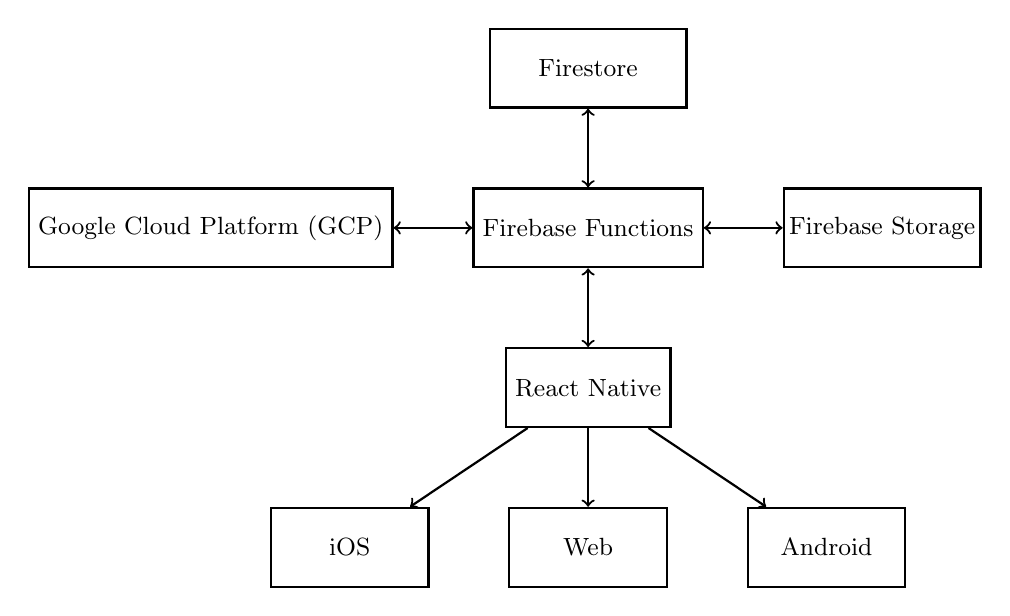
\begin{tikzpicture}[font=\small,thick]
 
% Start block
\node[draw,
    rectangle,
    minimum width=2.5cm,
    minimum height=1cm] (block1) {Firestore};
 
% Voltage and Current Measurement
\node[draw,
	rectangle,
    below=of block1,
    minimum width=2.5cm,
    minimum height=1cm
] (block2) { Firebase Functions };
 
% Power and voltage variation
\node[draw,
    left=of block2,
    minimum width=2.5cm,
    minimum height=1cm
] (block3) { Google Cloud Platform (GCP) };
 
 
\node[draw,
    rectangle,
    right=of block2,
    minimum height = 1cm,
    minimum width=2.5cm,
    inner sep=0] (block4) {Firebase Storage};
    
    
\node[draw,
	rectangle,
	below=of block2,
	minimum height = 1cm,
	minimum width=2cm
] (block5) {React Native};

\node[draw,
	rectangle,
	below=of block5,
	minimum height = 1cm,
	minimum width=2cm
] (block6) {Web};

\node[draw,
	rectangle,
	right=of block6,
	minimum height = 1cm,
	minimum width=2cm
] (block7) {Android};


\node[draw,
	rectangle,
	left=of block6,
	minimum height = 1cm,
	minimum width=2cm
] (block8) {iOS};
 
 
% Arrows
\draw[<->] (block1) edge (block2)
    (block2) edge (block3)
    (block2) edge (block4)
    (block2) edge (block5);
   
\draw[->]  (block5) edge (block6)
    (block5) edge (block7)
    (block5) edge (block8);
 
%\draw[-latex] (block4) -| (block5)
%    node[pos=0.25,fill=white,inner sep=0]{Yes};
% 
%\draw[-latex] (block4) -| (block6)
%    node[pos=0.25,fill=white,inner sep=0]{No};
 
%\draw[-latex] (block5) edge node[pos=0.4,fill=white,inner sep=2pt]{No}(block7)
%    (block5) -| (block8)
%        node[pos=0.25,fill=white,inner sep=0]{Yes};
% 
%\draw[-latex] (block6) edge node[pos=0.4,fill=white,inner sep=2pt]{No}(block9)
%    (block6) -| (block10)
%        node[pos=0.25,fill=white,inner sep=0]{Yes};
% 
%\draw (block7) |- (block12);
%\draw (block9) |- (block12);
%\draw (block8) |- (block7|-block12);
%\draw (block10) |- (block9|-block12);
%\draw[-latex] (block12) -- (block11);
 
\end{tikzpicture}
 
\end{document}
